%% Submissions for peer-review must enable line-numbering
%% using the lineno option in the \documentclass command.
%%
%% Preprints and camera-ready submissions do not need
%% line numbers, and should have this option removed.
%%
%% Please note that the line numbering option requires
%% version 1.1 or newer of the wlpeerj.cls file, and
%% the corresponding author info requires v1.2

\documentclass[fleqn,10pt,lineno]{wlpeerj} % for journal submissions

% ZNK -- Adding headers for pandoc

\setlength{\emergencystretch}{3em}
\providecommand{\tightlist}{
\setlength{\itemsep}{0pt}\setlength{\parskip}{0pt}}
\usepackage{lipsum}
\usepackage[unicode=true]{hyperref}
\usepackage{longtable}



\usepackage{lipsum} \usepackage{multirow}

\title{Application of a continuous lake trophic state index on lakes with limited data}

\author[1]{Farnaz Nojavan A.}

\corrauthor[1]{Farnaz Nojavan A.}{\href{mailto:f.nojavan@gmail.com}{\nolinkurl{f.nojavan@gmail.com}}}
\author[2]{Betty J. Kreakie}

\author[2]{Jeffrey W. Hollister}

\author[]{Song S. Qian}


\affil[1]{Farnaz's new affiliation address}
\affil[2]{US Environmental Protection Agency, Office of Research and Development, National Health and Environmental Effects Research Laboratory, Atlantic Ecology Division, 27 Tarzwell Drive Narragansett, RI, 02882, USA}
\affil[3]{Department of Environmental Sciences, The University of Toledo, Toledo, OH, United States}


%
% \author[1]{First Author}
% \author[2]{Second Author}
% \affil[1]{Address of first author}
% \affil[2]{Address of second author}
% \corrauthor[1]{First Author}{f.author@email.com}

% 

\begin{abstract}
Lake trophic state indices have long been used to provide a measure of the trophic state of lakes. Over time it has been determined that these indices perform better when they utilize multiple metrics and provide a continuous measurement of trophic state. We utilize such a method for trophic state that is based upon a Proportional Odds Logistic Regression (POLR) model and extend this model with a Bayesian multilevel model that predicts nutrient concentrations from universally available GIS data. This Bayesian multilevel model provides relatively accurate measures of trophic state and has an overall accuracy of 60\%. The approach illustrates a method for estimating a continuous, mutli-metric trophic state index for any lake in the United States. Future improvements to the model will focus on improving overall accuracy and use variables that are more sensitive to change over time.
% Dummy abstract text. Dummy abstract text. Dummy abstract text. Dummy abstract text. Dummy abstract text. Dummy abstract text. Dummy abstract text. Dummy abstract text. Dummy abstract text. Dummy abstract text. Dummy abstract text.
\end{abstract}

\begin{document}

\flushbottom
\maketitle
\thispagestyle{empty}

\hypertarget{introduction}{%
\section*{Introduction}\label{introduction}}
\addcontentsline{toc}{section}{Introduction}

In this brief research note, we extend a model for estimating a continuous multi-metric trophic state index described by Nojavan et al.~(n.d.). This model uses lake elevation and \emph{in situ} measurements of total nitrogen, total phosphorus, and secchi depth to provide a continuous index of trophic state. The drawback of the developed POLR model is the cost of monitoring multiple predictor variables (e.g., nutrients). This is addressed in the extended application by linking nitrogen and phosphorus to universally available GIS variables. The goal of the extended POLR model is to allow prediction of the trophic state of all lakes (i.e.~lakes with limited field data) in the United States.

\hypertarget{methods}{%
\section*{Methods}\label{methods}}
\addcontentsline{toc}{section}{Methods}

We present the extended application of the developed POLR model using a Bayesian multilevel model. Our modeling work flow is as follows:

\begin{enumerate}
\def\labelenumi{\arabic{enumi}.}
\tightlist
\item
  Develop a random forest model, using R's \texttt{randomForest} package, with 5000 trees using only GIS variables to identify the best predictor variables for nitrogen and phosphorus.
\item
  Develop the extended application model (the Bayesian multilevel model) using R's \texttt{rjags} package to run Just Another Gibbs Sampler (JAGS) from inside of R. JAGS is a program for simulation and analysis of Bayesian hierarchical models using Markov Chain Monte Carlo (MCMC).
\item
  Assess the performance of the extended application model using a hold-out validation method (90\% training set, 10\% evaluation set).
\end{enumerate}

We link nitrogen and phosphorus in the POLR model to a separate nutrient model built from universally available GIS data, thereby, avoiding the need for nitrogen and phosphorus data, costly variables to measure for all lakes. The number of variables for each response variable, nitrogen or phosphorus, was decided using random forest model's variable selection plots(Hollister, Milstead, and Kreakie 2016).

\hypertarget{results-and-discussion}{%
\section*{Results and Discussion}\label{results-and-discussion}}
\addcontentsline{toc}{section}{Results and Discussion}

Selected GIS variables for nitrogen and phosphorus were initially screened with variable selection plots (Figures \ref{fig:gis_vs_NTL} \& \ref{fig:gis_vs_PTL}).The figures show model mean squared error as a function of the number of variables. The best representation of nitrogen and phosphorus could be achieved using three variables, adding more than three variables had incremental (\(<0.1\)) impact on root mean square error. The three most important variables were ecoregion, \% evergreen forest, and latitude. The random forest models provided estimates of variable importance for nitrogen and phosphorus and the results are reported in figures \ref{fig:importancePlot_gis_NTL} \& \ref{fig:importancePlot_gis_PTL}.

Figure \ref{fig:DAG2} represents the regression models. The extended POLR model is grouped into two blocks (gray shaded rectangles). The trophic state classification regression, the POLR model in the lower block, includes nitrogen, phosphorus, secchi disk, and elevation as predictors. The nutrient model, in the upper block, estimates the means of nitrogen and phosphorus based on ecoregion, \% evergreen forest, and latitude. The two blocks are connected through the estimated means of nitrogen (\(\mu_{Nitrogen}\)) and phosphorus (\(\mu_{Phosphorus}\)) to form the combined model which enables trophic state classification for all lakes without the costly sampling requirement. The relationship between nitrogen, phosphorus, and their predictors was examined using multilevel linear regression models. The standard deviation of the normal distribution, as well as each parameter in the regression model, were then assigned non-informative prior distributions (uniform, or nearly so, to allow the information from the likelihood to be interpreted as a probability).

The three selected variables, latitude, eco-region, and \% evergreen forest, appear to be capturing patterns of total nutrient concentration at three different spatial scales.
Figures \ref{fig:PD_gisvs_N_Latitude} \& \ref{fig:PD_gisvs_P_Latitude} depict the partial dependency plot for latitude, the marginal effect of latitude on the predicted outcome of nitrogen or phosphorus in the random forest model. For example for predicted total nitrogen, high concentrations in the northern and southern extremes of the continental US and the lowest predicted concentrations correspond to the mid-latitudes. The ecoregion variable represents an intermediate scale among these three variables and represents the variation between the regions. Finally, the \% evergreen variable was summarized within a 3 kilometer buffer around each lake and is presumably summarizing more local land use decisions that are adjacent to lakes.

As mentioned, the extension of the developed POLR model uses eco-region, latitude, and watershed level \% evergreen forest as predictors for nitrogen and phosphorus. This contrasts with prior trophic state classification models that are applied to all lakes, regardless of the differences across scale. Lake trophic index, and hence lake trophic classes, should be calculated differently in different eco-regions to accommodate variation in landform and climate characteristics and our proposed model and extension bares this out by identifying and including and eco-regional approach to quantifying trophic state. Furthermore, the developed multilevel model structure can be further expanded to lake-specific trophic state index, upon availability of multiple measurements for each lake.

Mathematically, the models were set up as follows:

\begin{equation}
\mathrm{  \ Nitrogen_{ij}} \ \sim \ \mathcal{N}( \mu_{{Nitrogen}_{ij}},\sigma_{Nitrogen}^2)\\
\end{equation}
where \(\mu_{{Nitrogen}_{ij}}\) = \(X_{Nitrogen}B\), \(X_{Nitrogen}\) is the matrix of predictors, and \(B\) is the vector of coefficients. \(Nitrogen_{ij}\) is the \emph{i}th nitrogen observation in the \emph{j}th ecoregion.

\begin{equation}
\mathrm{  \ Phosphorus_{ij}} \ \sim \ \mathcal{N}( \mu_{{Phosphorus}_{ij}},\sigma_{Phosphorus}^2)\\
\end{equation}
where \(\mu_{{Phosphorus}_{ij}}\) = \(X_{Phosphorus}\Gamma\), \(X_{Phosphorus}\) is the matrix of predictors, and \(\Gamma\) is the vector of coefficients. \(Phosphorus_{ij}\) is the \emph{i}th phosphorus observation in the \emph{j}th ecoregion.

The overall accuracy of the extended POLR model was 0.6 and the balanced accuracies were 0.78, 0.77, 0.69, 0.68 for oligotrophic, mesotrophic, eutrophic, and hypereutrophic classes, respectively (Table \ref{tab:MultiPOLRCoeff}). Table \ref{tab:MultiPOLRCM} shows the confusion matrix for the extended POLR model.

The extended POLR model calculates lake trophic index and classes differently for different eco-regions. Please refer to Table \ref{tab:MultiPOLRCoeff} for varying coefficients in different eco-regions. For example, eco-regions 3, 6, and 5, corresponding to Northern Plains, Temperate Plains, and Southern Plains, have the highest positive coefficients for nitrogen. Hence, nitrogen plays a significant role in moving the trophic state index and class toward the eutrophic/hypereutrophic side of the trophic continuum. Further Table \ref{tab:MultiPOLRCoeff} shows the coefficients for latitude and \% evergreen. We included these predictors as they were selected as important variables by the random forest model. They may not help predictions dramatically but they do not hurt the results.

\hypertarget{tables}{%
\section*{Tables}\label{tables}}
\addcontentsline{toc}{section}{Tables}

\begin{table}[ht]
\caption {Coefficients for the extended POLR model.}
\label{tab:MultiPOLRCoeff}
\centering
 \begin{tabular}{llll}
  \hline
  &  & Mean & Standard Deviation\\ 
  \hline
  \multirow{3}{*}{\emph{Cutoff points/Thresholds}} & $C_{Oligo|Meso}$  & -156.60 & 44.04\\ 
  & $C_{Meso|Eu}$  & -6.18 & 8.29\\ 
  & $C_{Eu|Hyper}$ & 121.32 & 35.04\\ 
  \multirow{4}{*}{\emph{POLR model coefficients}}& $\alpha_{Elevation}$ & -40.20 & 12.86\\ 
  & $\alpha_{Nitrogen}$ & -44.33 & 29.29\\ 
  & $\alpha_{Phosphorus}$ & 165.90 & 46.96\\ 
  & $\alpha_{\text{Secchi Disk Depth}}$ & 0.18 & 5.23\\ 
  \multirow{11}{*}{\emph{Multilevel model coefficients for nitrogen}}& $\beta_{\%Evergreen}$ & 0.00 & 0.01\\ 
  & $\beta_{Ecoregion_1}$ & 0.34 & 0.13\\ 
  & $\beta_{Ecoregion_2}$ & -0.78 & 0.12\\ 
  & $\beta_{Ecoregion_3}$ & 0.96 & 0.15\\ 
  & $\beta_{Ecoregion_4}$ & -0.37 & 0.10\\ 
  & $\beta_{Ecoregion_5}$ & 0.59 & 0.10\\ 
  & $\beta_{Ecoregion_6}$ & 0.68 & 0.09\\ 
  & $\beta_{Ecoregion_7}$ & -0.01 & 0.10\\ 
  & $\beta_{Ecoregion_8}$ & -1.00 & 0.10\\ 
  & $\beta_{Ecoregion_9}$ & 0.11 & 0.12\\ 
  & $\beta_{Latitude}$ & 0.11 & 0.05\\ 
  \multirow{11}{*}{\emph{Multilevel model coefficients for phosphorus}}& $\gamma_{\%Evergreen}$ & -0.00 & 0.01\\ 
  & $\gamma_{Ecoregion_1}$ & 0.40 & 0.09\\ 
  & $\gamma_{Ecoregion_2}$ & -0.90 & 0.09\\ 
  & $\gamma_{Ecoregion_3}$ & 0.73 & 0.11\\ 
  & $\gamma_{Ecoregion_4}$ & -0.38 & 0.08\\ 
  & $\gamma_{Ecoregion_5}$ & 0.53 & 0.08\\ 
  & $\gamma_{Ecoregion_6}$ & 0.71 & 0.07\\ 
  & $\gamma_{Ecoregion_7}$ & -0.32 & 0.08\\ 
  & $\gamma_{Ecoregion_8}$ & -0.69 & 0.08\\ 
  & $\gamma_{Ecoregion_9}$ & 0.07 & 0.09\\ 
  & $\gamma_{Latitude}$ & -0.03 & 0.03\\ 
 {\emph{Logistic distribution's scale parameter}}& $\sigma$ & 75.64 & 21.27\\ 
  \hline
\end{tabular}
\end{table}

\begin{table}[ht]
\caption {Confusion matrix for multilevel POLR model. Each element of the matrix is the number of cases for which the actual state is the row and the predicted state is the column.}
\label{tab:MultiPOLRCM}
\centering
\begin{tabular}{lllll}
  \hline
 & Oligo & Meso & Eu & Hyper \\ 
  \hline
  Oligo & 5 & 3 & 0 & 0 \\
  Meso & 3 & 12 & 7 & 1 \\
  Eu & 0 & 0 & 16 & 10 \\
  Hyper & 0 & 1 & 3 & 9 \\
   \hline
\end{tabular}
\end{table}

\hypertarget{figures}{%
\section*{Figures}\label{figures}}
\addcontentsline{toc}{section}{Figures}

\begin{figure}
  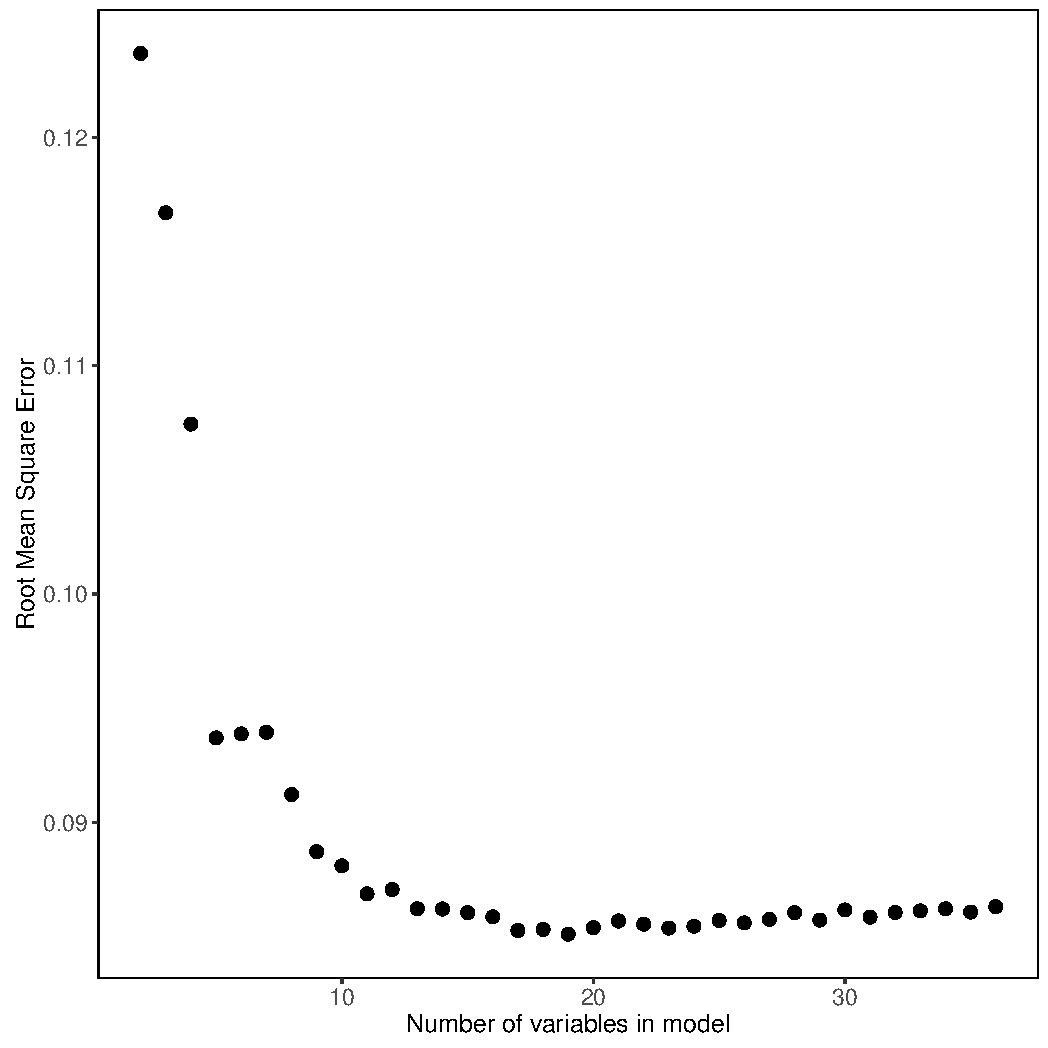
\includegraphics[scale=0.5]{gis_vs_NTL.pdf}
  \caption{Random Forest model's output for nitrogen with GIS only variables as predictors. Shows model mean squared error as a function of the number of variables.}
  \label{fig:gis_vs_NTL}
\end{figure}

\begin{figure}
  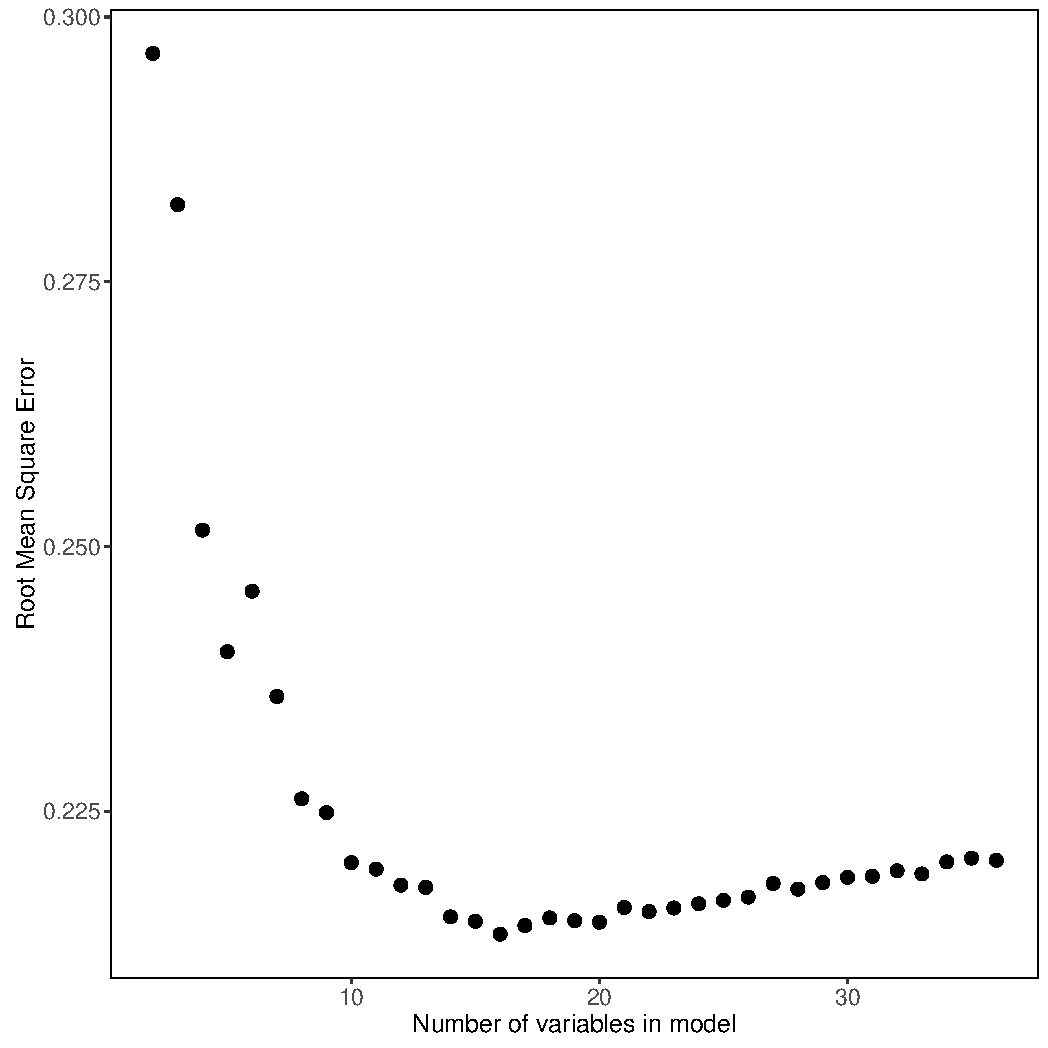
\includegraphics[scale=0.5]{gis_vs_PTL.pdf}
  \caption{Random Forest model's output for phosphorus with GIS only variables as predictors. Shows model mean squared error as a function of the number of variables.}
  \label{fig:gis_vs_PTL}
\end{figure}

\begin{figure}
  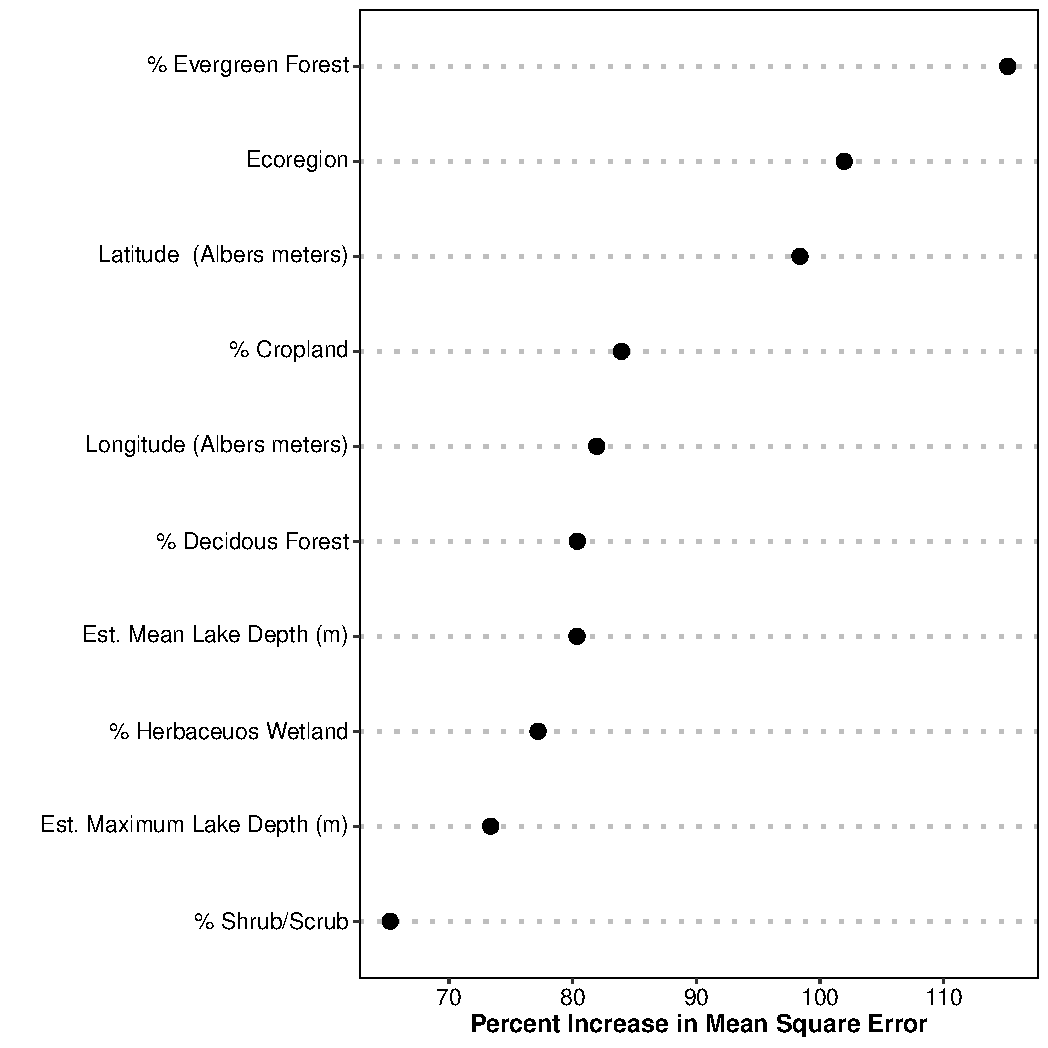
\includegraphics[width=\textwidth]{importanceplot_gis_NTL.pdf}
  \caption{Random Forest model's output for nitrogen predictors. Importance plot for GIS variables. Shows percent increase in mean squared error. Higher values of percent increase in mean squared error indicates higher importance.}
  \label{fig:importancePlot_gis_NTL}
\end{figure}

\begin{figure}
  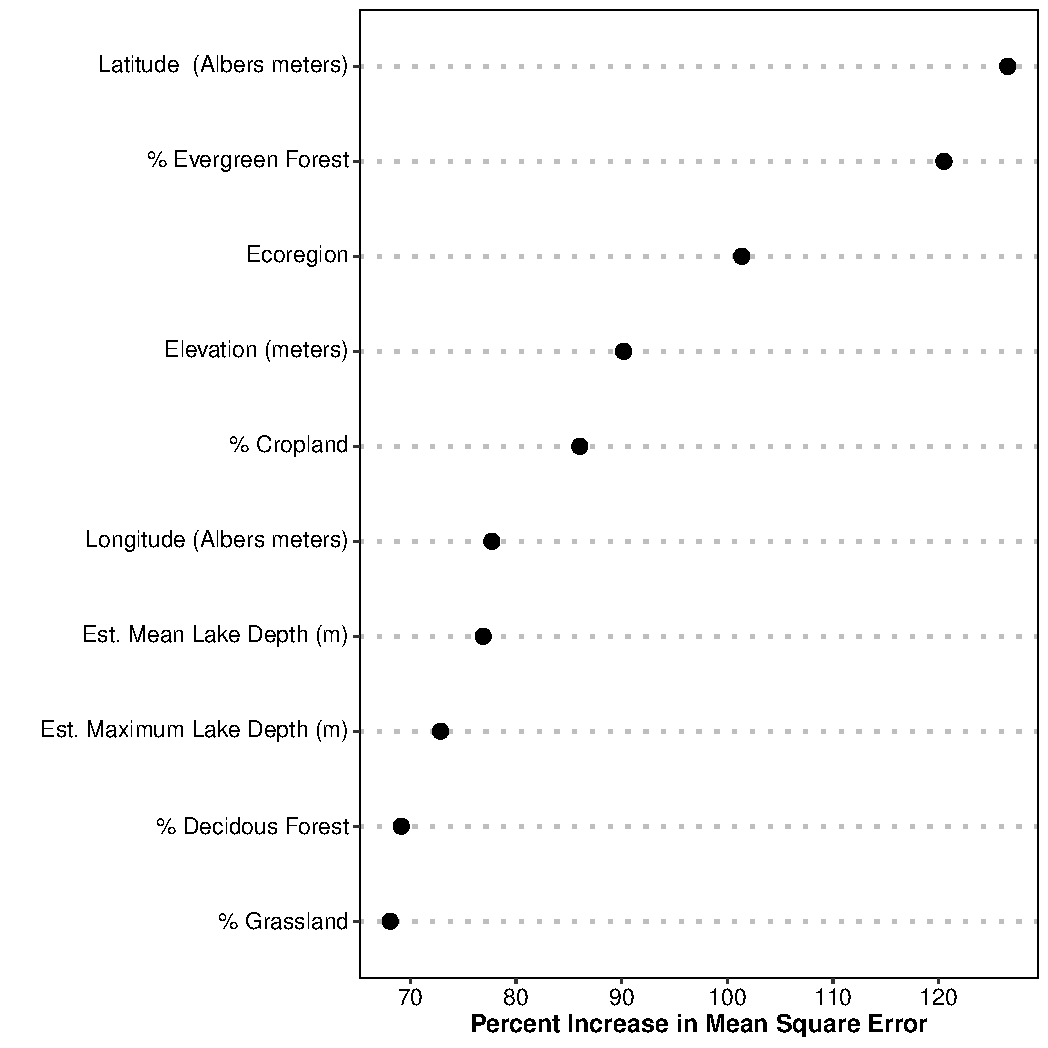
\includegraphics[width=\textwidth]{importanceplot_gis_PTL.pdf}
  \caption{Random Forest model's output for nitrogen predictors. Importance plot for GIS variables. Shows percent increase in mean squared error. Higher values of percent increase in mean squared error indicates higher importance.}
  \label{fig:importancePlot_gis_PTL}
\end{figure}

\begin{figure}
  \includegraphics[page=4, scale=0.85, trim=20mm 45mm 0mm 45mm, clip]{cyanobacteria-dag-model1.pdf}
  \caption{Directed Acyclic Graphical (DAG) model. The lower box depicts the POLR model with its four predictors of secchi disk depth (SDD), elevation, nitrogen, and phosphorus. The upper box is the extension to the POLR model to predict nitrogen and phosphorus using universally available GIS variables.}
  \label{fig:DAG2}
\end{figure}

\begin{figure}
  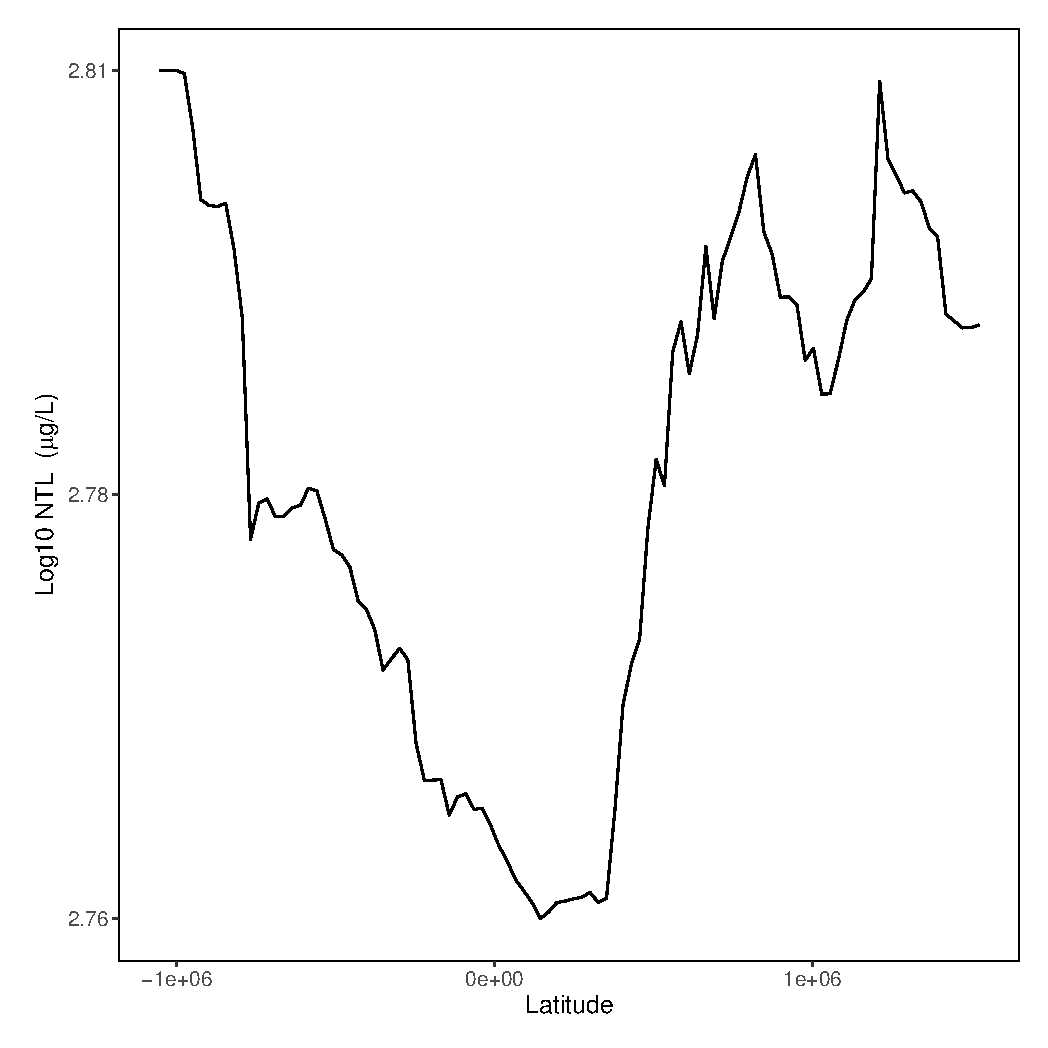
\includegraphics[scale=0.5]{PD_gisvs_N_Latitude.pdf}
  \caption{Partial dependency plot for predicted total nitrogen over the range latitude: the effect of latitude on predicted total nitrogen when the rest of the predictors are held constant.}
  \label{fig:PD_gisvs_N_Latitude}
\end{figure}

\begin{figure}
  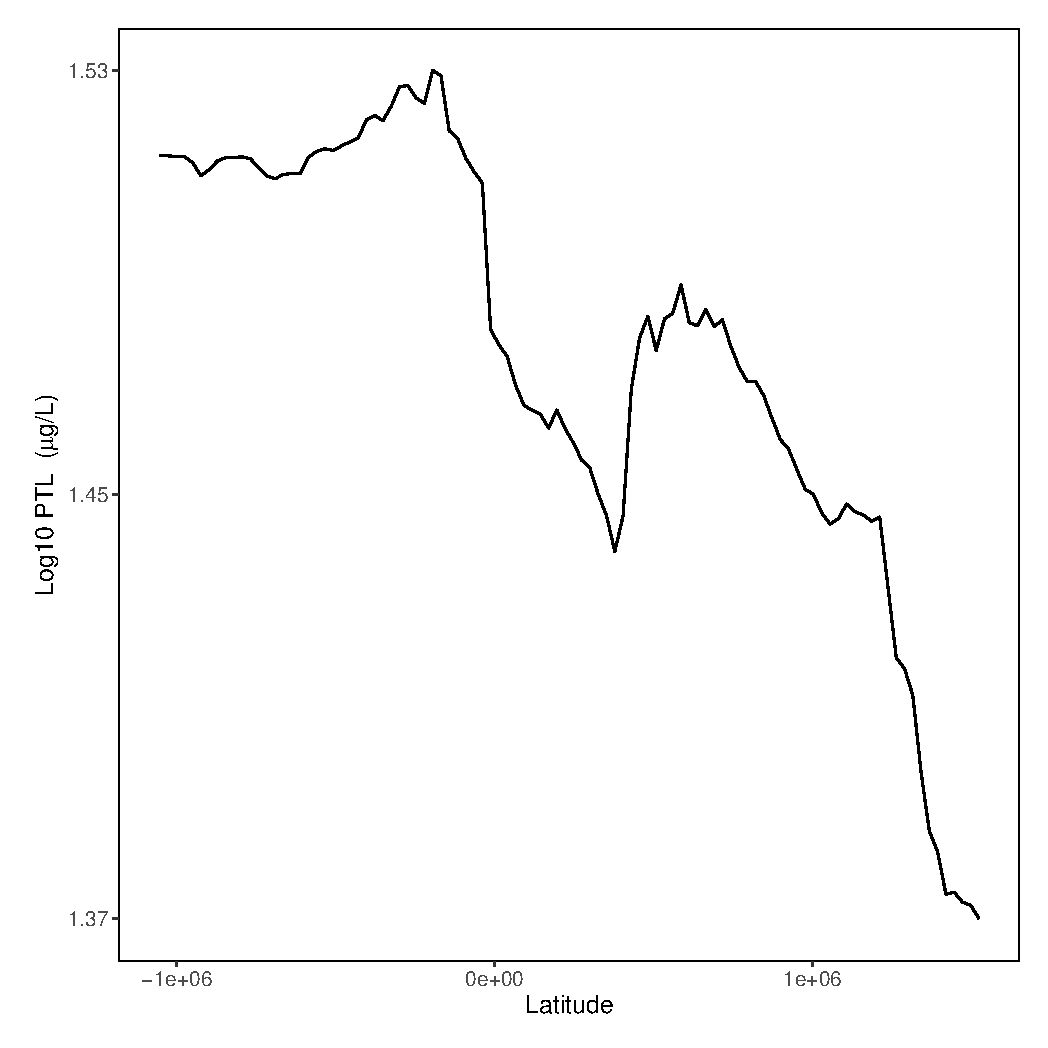
\includegraphics[scale=0.5]{PD_gisvs_P_Latitude.pdf}
  \caption{Partial dependency plot for predicted total phosphorus over the range latitude: the effect of latitude on predicted total phosphorus when the rest of the predictors are held constant.}
  \label{fig:PD_gisvs_P_Latitude}
\end{figure}

\hypertarget{references}{%
\section*{References}\label{references}}
\addcontentsline{toc}{section}{References}

\bibliography{ReferencesSup}

\hypertarget{refs}{}
\leavevmode\hypertarget{ref-hollister2016modeling}{}%
Hollister, Jeffrey W, W Bryan Milstead, and Betty J Kreakie. 2016. ``Modeling Lake Trophic State: A Random Forest Approach.'' \emph{Ecosphere} 7 (3).

\leavevmode\hypertarget{ref-nojavantsi}{}%
Nojavan A., Farnaz, Betty J. Kreakie, Hollister Jeffrey W., and Song Qian. n.d. ``Rethinking the Lake Trophic State Index.'' \emph{PeerJ}.



\end{document}
